\documentclass[12pt]{article}
\usepackage[utf8]{inputenc}
\usepackage{float}
\usepackage{amsmath}


\usepackage[hmargin=3cm,vmargin=6.0cm]{geometry}
\topmargin=-2cm
\addtolength{\textheight}{6.5cm}
\addtolength{\textwidth}{2.0cm}
\setlength{\oddsidemargin}{0.0cm}
\setlength{\evensidemargin}{0.0cm}
\usepackage{indentfirst}
\usepackage{amsfonts}
\usepackage{graphicx}


\begin{document}

\section*{Student Information}

Name : Abdulkadir Pamukçu\\

ID : 2237774


\section*{Answer 1}

\subsection*{a)}
Since the sample sizes are small (i.e., n1< 30 and n2< 30), the confidence interval formula with t is appropriate\\
Our variables are those:\\ 1st Sample size $\rightarrow$ $n_1$ = 19  1st Sample mean $\rightarrow$ $\Bar{x_2}$ = 3.375 1s Standart deviation $\rightarrow$ s$_1$ = 0.96 \\
\\
2nd Sample size $\rightarrow$ $n_2$ = 15  2nd Sample mean $\rightarrow$ $\Bar{x_2}$ = 2.05 2nd Standart deviation $\rightarrow$ s$_2$ = 1.12\\
 
We need to compute S$_p$, the pooled estimate of the common standard deviation.
 
S$_p$ = $\sqrt{ ((n_1 -1)(s_1)^2 + (n_2 - 1)(s_2)^2)  / ( n_1 + n_2 - 2)    }   $\\
 \\
S$_p$ = 1.0330\\
\\
Sp is falling in between the standard deviations in the two groups. The degrees of freedom (df) = $n_1$ + $n_2$ - 2  = 19+15-2 = 32. To $\%$95 confidence interval $\alpha$ = 0.05 and t is 2.037 from the t-Table A5 at the book. \\
\\
Then computation is follows like that:\\

$\Bar{x_1}$- $\Bar{x_2}$ $\pm$  t  S$_p$ $\sqrt{1/ n_1 + 1/n_2}$\\
\\
Put the values for both equation:\\

3.375 - 2.05 +  2.037 $\times$ 1.0330 $\times$ $\sqrt{1/ 19 + 1/15}$ = 2.051\\
\\
3.375 - 2.05 -  2.037 $\times$ 1.0330 $\times$ $\sqrt{1/ 19 + 1/15}$ = 0.598\\

So the $\%$95 confidence interval for the difference is [0.598, 2.051]\\

\subsection*{b)} 

Since we did all the calculations in subsection-a we are not gonna do it again.\\
This time our t is 1.694 since $\alpha$ = 0.1 since to have confidence interval $\%$90\\

Then computation is follows like that:\\

$\Bar{x_1}$- $\Bar{x_2}$ $\pm$  t  S$_p$ $\sqrt{1/ n_1 + 1/n_2}$\\
Put the values for both equation:\\

3.375 - 2.05 +  1.679 $\times$ 1.0330 $\times$ $\sqrt{1/ 19 + 1/15}$ = 1.924\\
3.375 - 2.05 -  1.679 $\times$ 1.0330 $\times$ $\sqrt{1/ 19 + 1/15}$ = 0.725\\

So the $\%$95 confidence interval for the difference is [0.725, 1.924]\\

\subsection*{c)}

We need to find the confidence interval of people with age 40 and above supports with confidence level $\%$95 \\
Confident interval for the mean is:\\
\\
 $\Bar{x}$ $\pm$ t$_(a/2)$ $\times$ S $\sqrt{n}$   

We already now the standart deviance of the elder group. S = 0.96 \\
And mean of the sample is $\Bar{x}$ = 3.375\\
We can find t$_(a/2)$ from the table 5a at the book. df (degrees of freedom) is n-1 = 18 and $\alpha$ = 0.05\\
So t$_(a/2)$ = 2.101\\
\\

So confident interval is: [2.912, 3.837].

The confidence interval with confidence level of $\%$95 is not always over 3 we can not say that age 40 and above supports BREXIT with $\%$95 confidence level.\\


\section*{Answer 2}

\subsection*{a)}
As given in the question 20.00 kg olympic bars being produced. \\
From that we can state the null hypothesis:\\
$H_0$ : $\mu$ = 20.00\\


\subsection*{b)}
If product have different weight than 20.00 kg it is not qualified. Also the alternative hypothesis is mathematical opposite of the null hypothesis. \\
So, we can state the alternative hypothesis:\\
$H_a$ : $\mu$ $\neq$ 20.00\\

\subsection*{c)}

We are going to find test statistic t by using t-test formula t-test formula to draw t- test diagram.\\

Our variables are those:\\ Sample average $\rightarrow$ $\Bar{x}$ = 20.7  Expected mean $\rightarrow$  $\mu_0$ = 20 Standart deviation $\rightarrow$ s = 0.07. Also $\alpha$ = 0.01 is can be deriven from the question. ( statistical significance ) \\
\\
The test formula is below:\\
\\
t = ($\Bar{x}$ - $\mu_0$) / (s / $\sqrt{n}$)\\
So, t = 3.317\\
\\
Then, we need to find the rejection region to draw the t-test diagram and find out the answer of question. \\
Degrees of freedom is n - 1 = 11 - 1 = 10 and $\alpha$ = 0.01\\ 
By using these we can find the t$_(a/2)$ from the t-table 5a from the book.\\
t$_(a/2)$ = 3.168\\
So the diagram is:\\
\\\
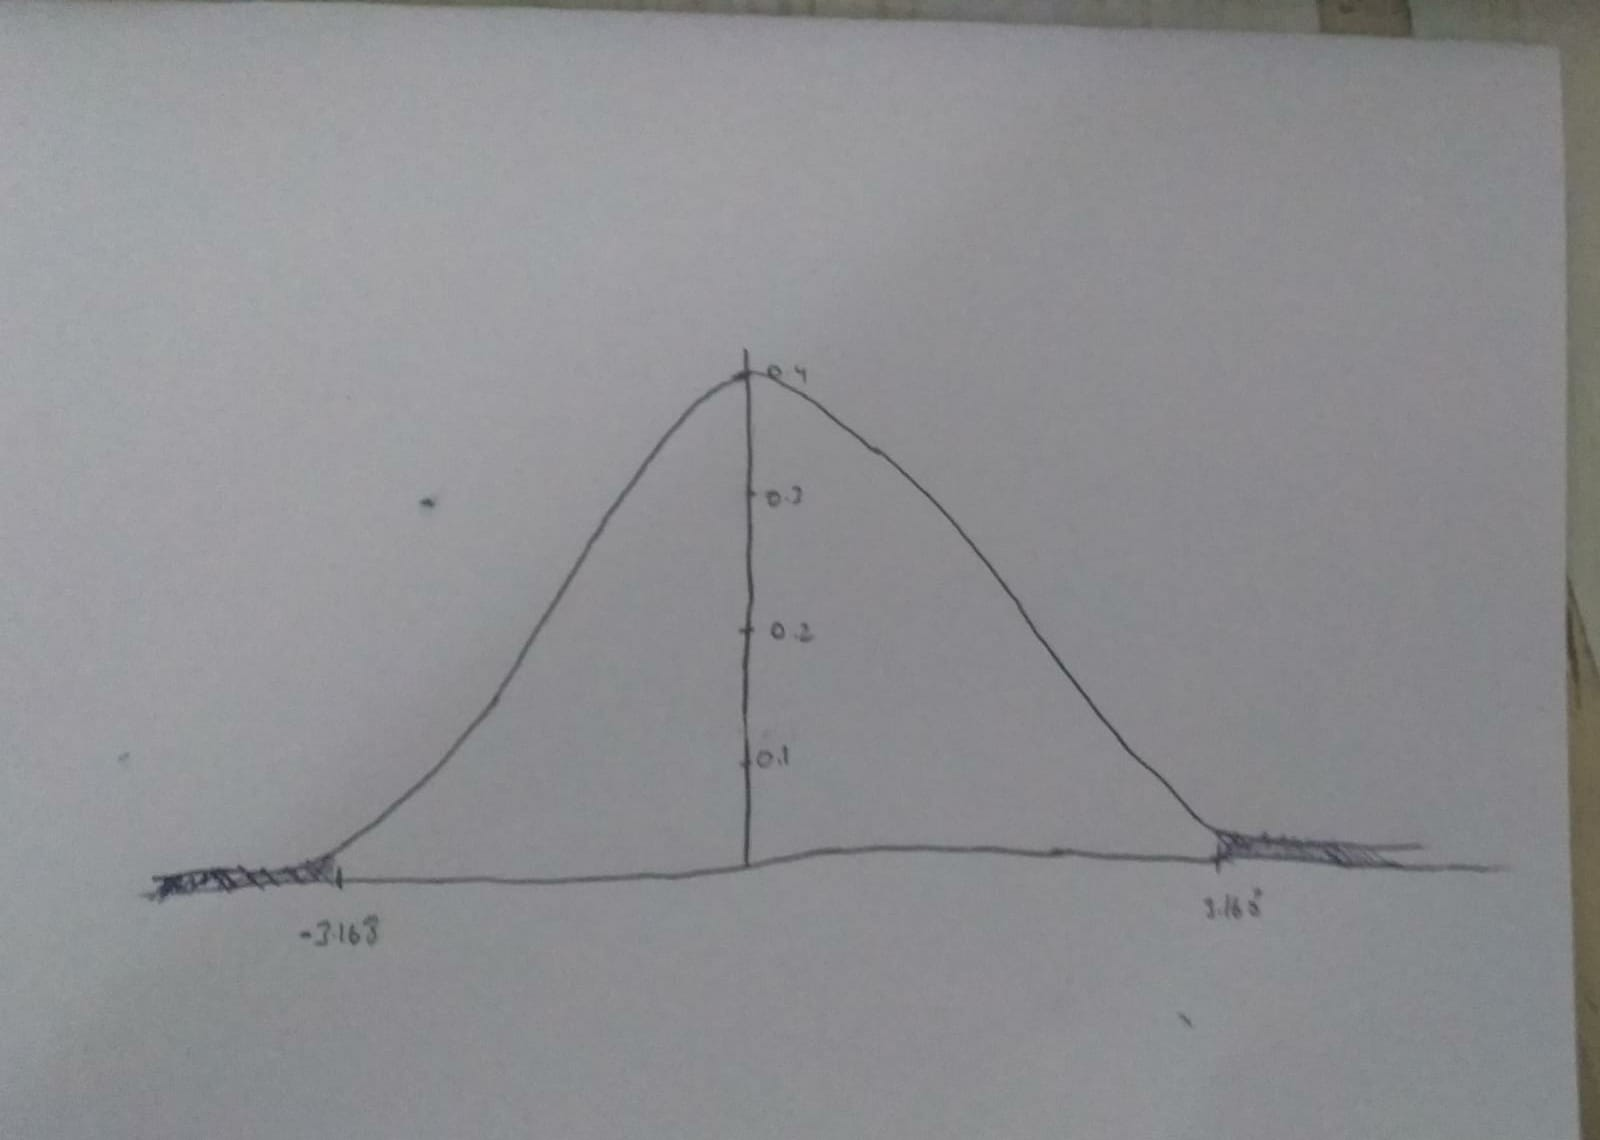
\includegraphics[width=14cm, height=7cm]{diagram1}\\
\\ 
The painted areas indicates the rejection regions. It is(-$\infty$, -3.169] $\cup$ [3.169,$\infty$).\\
\\
Now, we can clearly observe the fact that the test statistic t locates in rejection region. (3.316)\\
\\
So, the null hypothesis got rejected. Hence, they should stop the production and check the line.\\

 
    
\section*{Answer 3}

\subsection*{a)}
Lets call existing painkiller drugs in market A and the new claimed to-be superior drug B. \\
Null hypothesis is stated as: \\
$H_0$ : $\mu_A$ =$\mu_B$\\

\subsection*{b)}
Lets call existing painkiller drugs in market A and the new claimed to-be superior drug B. \\
Alternate hypothesis is stated as: \\
$H_0$ : $\mu_A$ < $\mu_A$\\

\subsection*{c)}

We are going to use z formula formula to draw z-test diagram.\\

Our variables are those:\\ Mean $\rightarrow$ $\mu_0$ = 3. Standart deviation $\rightarrow$ $\sigma$ = 1.4. Also $\rho$ = 0.05 is can be deriven from the question. ( level of significance ) \\
\\
The test formula is below:\\
\\
Z = ($\mu$ - $\mu_0$) / ($\sigma$ / $\sqrt{n}$ ) \\
\\
So Z = -1.18\\
\\
Also we know the z$(_0.05)$ = 1.644 from the book. We are ready to draw the diagram.\\
\\
So the diagram is:\\
\\
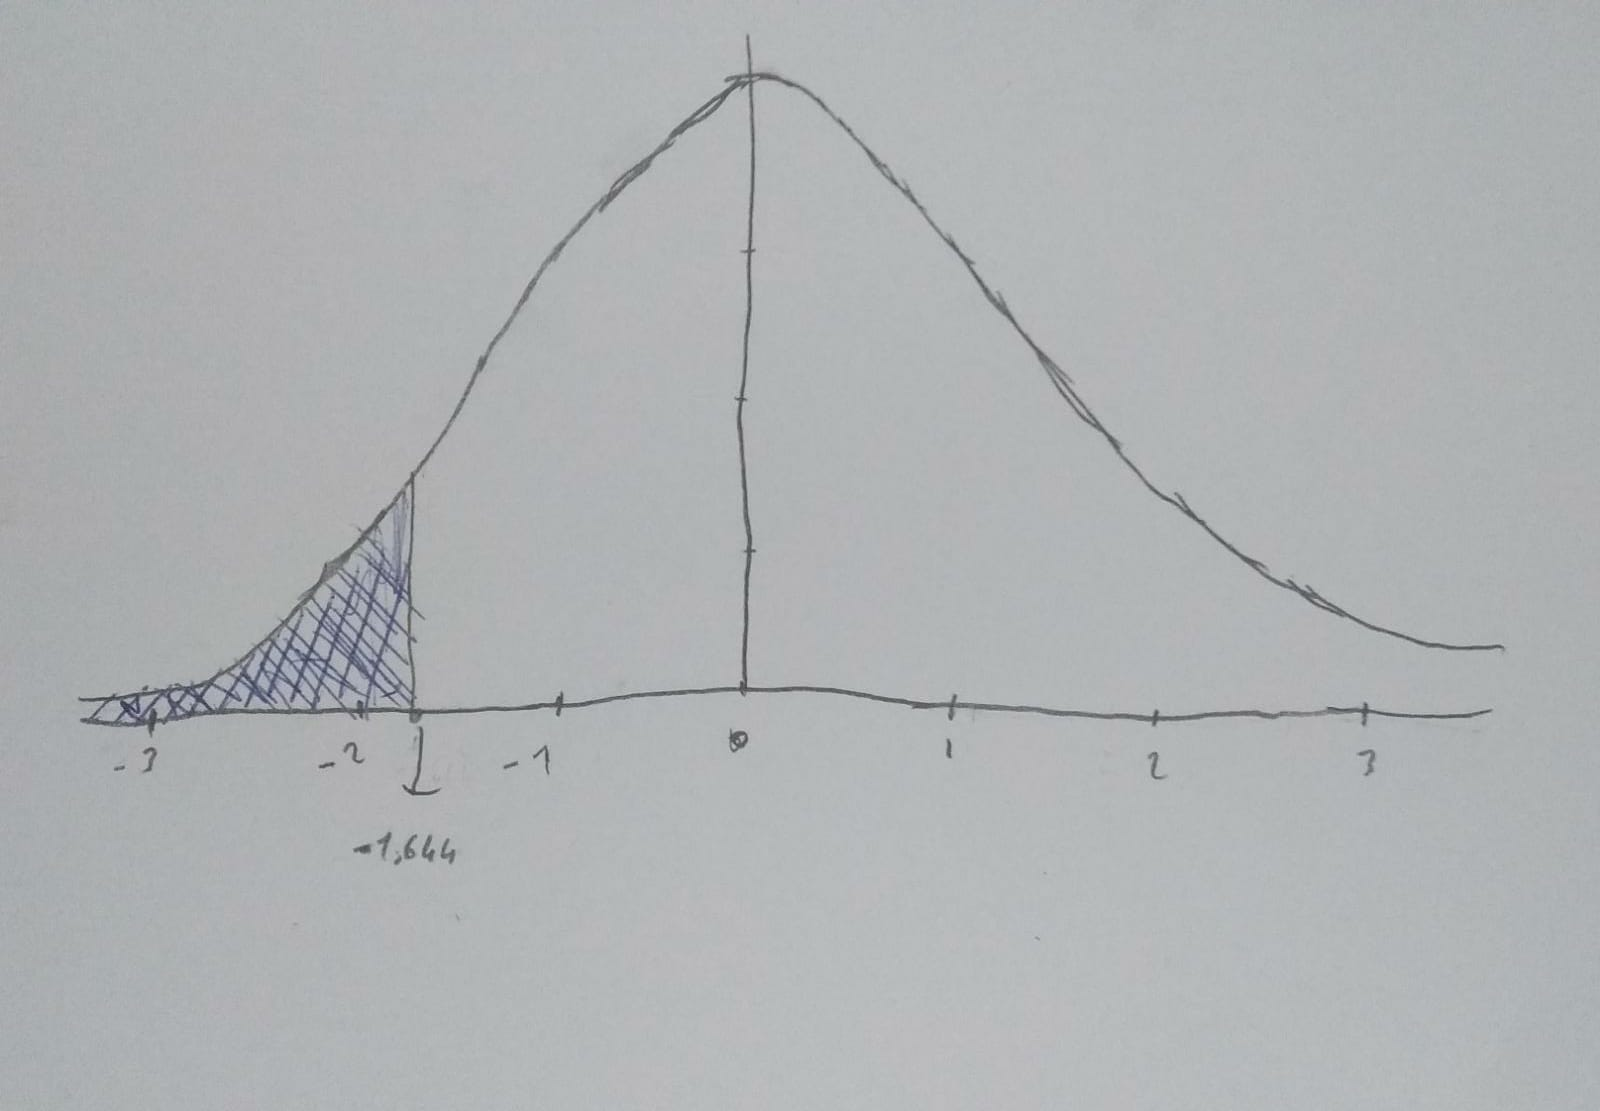
\includegraphics[width=14cm, height=7cm]{diagram2}\\
\\
The painted areas indicates the rejection regions.\\
\\
Because of the the z value that observed does not reside in the rejection region, we can't state that new painkiller drug really produce better results.\\





\end{document}

